\documentclass[11pt]{article}
\usepackage[margin=1in]{geometry}
\usepackage{amsmath,amssymb,amsfonts}
\usepackage{graphicx, float}
\usepackage{fancyhdr,booktabs}
\usepackage{listings}
\usepackage[normalem]{ulem}
\lstset{
    language=Python,
    basicstyle=\ttfamily\small,
    breaklines=true,
    keepspaces=true,
    showstringspaces=false
}

\renewcommand{\labelitemi}{$\bullet$}
\renewcommand{\labelitemii}{$\circ$}
\renewcommand{\labelitemiii}{$\rightarrow$}
\renewcommand{\labelitemiv}{$\cdot$}

% Header and Footer Setup
\pagestyle{fancy}
\fancyhf{}
\lhead{Ph429 NLD \& Chaos -- Fall 2026}
\rhead{Problem Set 3}
\cfoot{\thepage}

\title{\textbf{Ph429: Nonlinear Dynamics \& Chaos}\\[0.5ex]\Large Problem Set 3}
\author{Zeshui Song}
\date{Fall 2026}

\begin{document}
\maketitle

\vspace{-1em}
\subsection*{Problem 1}
\textit{(Problems 3.4.5--10 in Strogatz)}\\
For the following systems, find the values of $r$ at which bifurcations occur, classify the bifurcation as saddle-node, transcritical, or (super- or sub-critical) pitchfork, and sketch the bifurcation diagram of fixed points $x^*$ as a function of $r$.\\\\
If possible, describe how or perform the finding of the normal form for each.

\begin{enumerate}
    % The handout labels the first two systems (b); the first is treated as (a).
    \item[(a)] \[\dot{x} = r - 3x^2\]
    \paragraph{Solution}\mbox{} 
    \begin{itemize}
        \item Find fixed points:
        \[\dot{x} = f(x)\quad \implies f(x^*) = 0\]
        \[r-3{x^*}^2=0\]
        \[x^* = \pm\sqrt{\frac{r}{3}}\]
        \item Vary parameter $r$ and find bifurcation points:
        \begin{itemize}
            \item $r<0$: No fixed points
            \item $r=0$: One fixed point at $x^*=0$ 
            \item $r>0$: Two fixed points at $x^* = \pm\sqrt{\frac{r}{3}}$
        \end{itemize}
        Since the number of fixed points changes from 0 to 2 at $r=0$, this is a saddle-node bifurcation with a \underline{bifurcation point at $x^*=0,\,r=0$}.
        \item Find stability of fixed points:
        \[f'(x) = -6x\]
        \begin{itemize}
            \item $r=0$: $f'(x^*)=f'(0)=0$ (inconclusive)
            \item $r>0$:
            \begin{itemize}
                \item $x^* = +\sqrt{\frac{r}{3}}$: $f'(x^*) < 0$ (stable)
                \item $x^* = -\sqrt{\frac{r}{3}}$: $f'(x^*) > 0$ (unstable)
            \end{itemize}
        \end{itemize}
        \newpage
        \item Bifurcation diagram:
        \begin{center}
            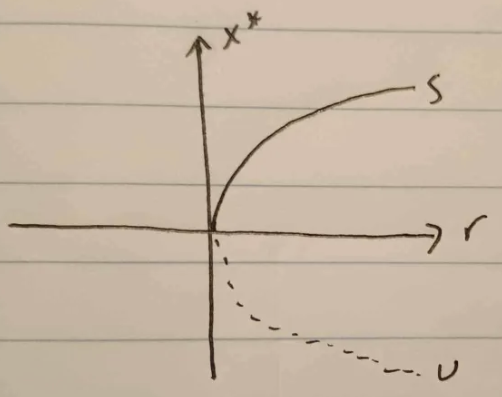
\includegraphics[width=0.5\textwidth]{p1a.png}
        \end{center}
        \item Normal form: rescale $x$ and $r$ to get $\dot{x} = r - x^2$.
        \[3\dot{x} = 3r - 9x^2\]
        Let $y = 3x$, $\mu = 3r$
        \[\implies \dot{y} = \mu - y^2\]
    \end{itemize}

    \item[(b)] \[\dot{x} = rx - \frac{x}{1+x}\]
    \paragraph{Solution}\mbox{} 
    \begin{itemize}
        \item Find fixed points:
        \[\dot{x} = f(x)\quad \implies f(x^*) = 0\]
        \[x^*\left(r - \frac{1}{1+x^*}\right)=0\]
        \[x^* = 0,\quad x^* = \frac{1}{r}-1\]
        \item Vary parameter $r$ and find bifurcation points:
        \begin{itemize}
            \item $r<1$: Two fixed points $x^* = 0,\quad x^* = \frac{1}{r}-1$
            \item $r = 1$: One fixed point $x^* = 0$
            \item $r>1$: Two fixed points $x^* = 0,\quad x^* = \frac{1}{r}-1$
        \end{itemize}
        \item Find stability of fixed points:
        \[f'(x) = r-\frac{(1+x)-x}{(1+x)^2}=r-\frac{1}{(1+x)^2}\]
        \[f'(0) = r-1\]
        \[f'\left(\frac{1}{r}-1\right) = r-\frac{1}{\left(1+\frac{1}{r}-1\right)^2} = r-\frac{1}{\left(\frac{1}{r}\right)^2} = r-r^2 = r(1-r)\]
        \newpage
        \begin{itemize}
            \item $r<0$:
            \begin{itemize}
                \item $x^* = 0:$ $f(x^*)<0$ (stable)
                \item $x^* = \frac{1}{r}-1$: $f(x^*)<0$ (stable)
            \end{itemize}
            \item $0<r<1$: 
            \begin{itemize}
                \item $x^* = 0:$ $f(x^*)<0$ (stable)
                \item $x^* = \frac{1}{r}-1$: $f(x^*)>0$ (unstable)
            \end{itemize}
            \item $r = 1$:
            \begin{itemize}
                \item $x^*=0:$ $f(x^*)=0$ (inconclusive)
            \end{itemize}
            \item $r>1$:
            \begin{itemize}
                \item $x^* = 0:$ $f(x^*)>0$ (unstable)
                \item $x^* = \frac{1}{r}-1:$ $f(x^*)<0$ (stable)
            \end{itemize}
            Note that $r\to0$ causes $x^*= \frac{1}{r}-1 \to \infty$. Also, the original equation is not defined at $x=-1$.\\\\
            \underline{This is a transcritical bifurcation at $x^* =0,\,r=1$}
        \end{itemize}
        \item Bifurcation diagram: (RHP)
        \begin{center}
            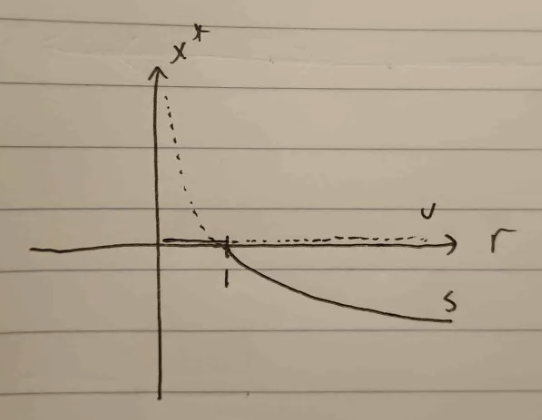
\includegraphics[width=0.5\textwidth]{p1b.png}
        \end{center}
        \item Normal form: Using taylor series expansion around the bifurcation point $x^*=0$
        \[\dot{x} = rx - \frac{x}{1+x} \approx rx-x(1-x+x^2- \ldots)\]
        Neglecting higher order terms, we have
        \[\dot{x} \approx rx - x + x^2 = (r-1)x + x^2\]
        Let $\mu = r-1$, we have
        \[\dot{x} = \mu x + x^2\]
    \end{itemize}
\newpage
    \item[(c)] \[\dot{x} = 5 - re^{-x^2}\]
    \paragraph{Solution}\mbox{} 
        \begin{itemize}
        \item Find fixed points:
        \[\dot{x} = f(x)\quad \implies f(x^*) = 0\]
        \[5 - re^{-{x^*}^2} = 0\implies e^{-{x^*}^2} =\frac{5}{r} \implies {x^*}^2 = -\ln\left(\frac{5}{r}\right)\]
        \[x^* = \pm \sqrt{\ln\left(\frac{r}{5}\right)}\]
        \item Vary parameter $r$ and find bifurcation points:\\
        For real fixed points, $r/5 \geq 1 \implies r \geq 5$ so that $\ln(r/5) \geq 0$. 
        \begin{itemize}
            \item $r<5$: No fixed points 
            \item $r=5$: One fixed point at $x^*=0$ 
            \item $r>5$: Two fixed points at $x^* = \pm \sqrt{\ln\left(\frac{r}{5}\right)}$
        \end{itemize}
        \item Find stability of fixed points:
        \[f'(x) = 2rxe^{-x^2}\]
        \begin{itemize}
            \item $r=5$:
            \begin{itemize}
                \item $x^*=0:$ $f'(x^*)=0$ (inconclusive)
            \end{itemize}
            \item $r>5$:
            \begin{itemize}
                \item $x^* = -\sqrt{\ln\left(\frac{r}{5}\right)}$: $f'(x^*)<0$ (stable)
                \item $x^* = \sqrt{\ln\left(\frac{r}{5}\right)}$: $f'(x^*)>0$ (unstable)
            \end{itemize}
        \end{itemize}
            Since we go from 0 fixed points to 2 fixed points at $r=5$, this is a \uline{saddle-node bifurcation at $x^*=0, \,r=5$}.  
        \item Bifurcation diagram:
        \begin{center}
            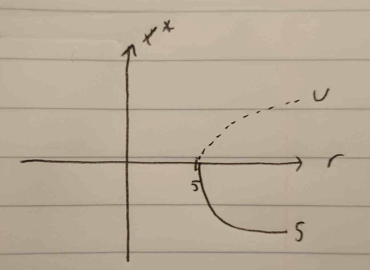
\includegraphics[width=0.5\textwidth]{p1c.png}
        \end{center}
        \item Normal form: $\dot{x} = r+x^2$. Rewriting using a taylor series around the bifurcation point $x^*=0$ and $r=5$, we have:
        \[\dot{x} = 5 - re^{-x^2}\approx 5 - r\left(1-x^2+\frac{x^4}{2}-\ldots\right)\]
        Neglecting higher order terms, we have
        \[\dot{x} \approx 5 - r + rx^2 = (5-r) + rx^2\]
        Let $\mu = 5-r$, and $r\approx 5$ near the bifurcation:
        \[\dot{x} = \mu + 5x^2\]
        
    \end{itemize}

    \item[(d)] \[\dot{x} = rx - \frac{x}{1+x^2}\]
    \paragraph{Solution}\mbox{} 
    \begin{itemize}
        \item Find fixed points:
        \[\dot{x} = f(x)\quad \implies f(x^*) = 0\]
        \[x^*\left(r - \frac{1}{1+{x^*}^2}\right) = 0\]
        \[x^* = 0,\quad x^*=\pm\sqrt{\frac{1}{r}-1}\]
        \item Vary parameter $r$ and find bifurcation points:\\
        For real fixed points $\frac{1}{r}-1 \geq 0 \implies 0<r\leq 1$.
        \begin{itemize}

            \item $r<0$: One fixed point $x^* = 0$
            \item $0<r<1$: Three fixed points $x^* = 0,\quad x^* = \pm\sqrt{\frac{1}{r}-1}$
            \item $r>1$: One fixed point $x^* = 0$
        \end{itemize}
        \item Find stability of fixed points:
        \[f'(x) = r-\frac{(1+x^2)-x(2x)}{(1+x^2)^2} = r - \frac{1-x^2 }{(1+x^2)^2}\]
        \[f'(0) = r-1\]
        \[f'\left(\pm\sqrt{\frac{1}{r}-1}\right) 
        = r - \frac{1-\left(\frac{1}{r}-1\right)}{\left(1+\frac{1}{r}-1\right)^2} 
        = r - \frac{2-\frac{1}{r}}{\left(\frac{1}{r}\right)^2} 
        = r - (2r^2 -r) = 2r - 2r^2 = 2r(1-r)\]
        \begin{itemize}
            \item $r<0$: 
            \begin{itemize}
                \item $x^* = 0$: $f'(x^*)<0$ (stable)
            \end{itemize}
            \item $r=0$:
            \begin{itemize}
                \item $x^* = 0$: $f'(x^*)<0$ (stable)
            \end{itemize}
            \item $0<r<1$:
            \begin{itemize}
                \item $x^* = 0$: $f'(x^*)<0$ (stable)
                \item $x^* = -\sqrt{\frac{1}{r}-1}$: $f'(x^*)>0$ (unstable)
                \item $x^* = \sqrt{\frac{1}{r}-1}$: $f'(x^*)>0$ (unstable)
            \end{itemize}
            \item $r=1$:
            \begin{itemize}
                \item $x^* = 0$: $f'(x^*)=0$ (inconclusive)
            \end{itemize}
            \item $r>1$:
            \begin{itemize}
                \item $x^* = 0$: $f'(x^*)>0$ (unstable)
            \end{itemize}
        \end{itemize}
        Since we go from 3 fixed points to 1 fixed point where the two symmetrical fixed points are unstable while the middle one is stable, this is a \uline{subcritical pitchfork bifurcation at $x^*=0,\,r=1$}
        \item Bifurcation diagram:
        \begin{center}
            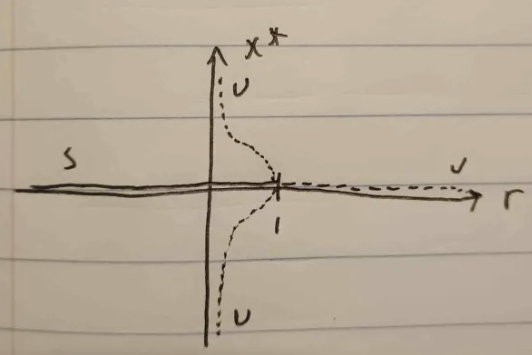
\includegraphics[width=0.5\textwidth]{p1d.png}
        \end{center}
        \item Normal form: $\dot{x}=rx+x^3$. Rewriting using a taylor series around the bifurcation point $x^*=0$ and $r=1$, we have:
        \[\dot{x}= rx-\frac{x}{1+x^2} \approx rx - x(1-x^2+x^4-\ldots)\]
        Neglecting higher order terms, we have
        \[\dot{x} \approx rx - x + x^3 = (r-1)x + x^3\]
        Let $\mu = r-1$, we have
        \[\dot{x} = \mu x + x^3\]
    \end{itemize}
    \item[(e)] \[\dot{x} = x + \tanh(rx)\]
    \paragraph{Solution}\mbox{} 
    \begin{itemize}
        \item Find fixed points:
        \[\dot{x} = f(x)\quad \implies f(x^*) = 0\]
        \[x^* + \tanh(rx^*) = 0\]
        One fixed point is $x^*=0$. Graphically, it can be seen that two other fixed points appear for some $r<0$:
        \begin{center}
            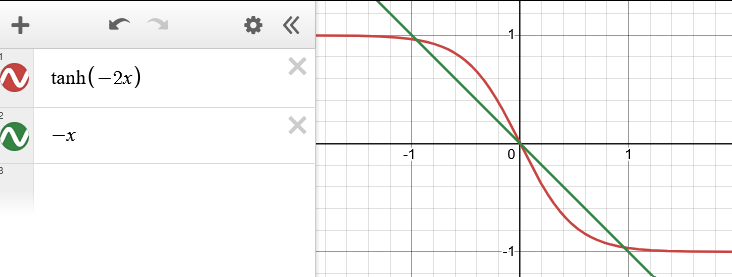
\includegraphics[width=0.5\textwidth]{p1e.png}
        \end{center}
        \item Since we can't solve for the other fixed points explicitly, I can try finding a bifurcation point based on the assumption that this is some form of subcritical pitchfork bifurcation. Since we start with one fixed point but it becomes three fixed points as $r$ decreases.\\\\
        Find $r$ where the fixed point at $x^*=0$ changes stability:
        \[f'(x) = 1 + r \,sech^2(rx)\]
        \[f'(0) = 1 + r\]
        For $r<-1$, the fixed point at $x^*=0$ is stable, and for $r>-1$, it is unstable. Therefore, the candidate bifurcation point is at $r=-1$.
        \item Verify using a taylor series expansion around the candidate bifurcation point $x^*=0$ and $r=-1$:
        \[f(x) = x + \tanh(rx) \approx x + \left(rx - \frac{(rx)^3}{3} + \frac{(rx)^5}{5} - \ldots\right)\]
        Neglecting higher order terms, we have
        \[f(x) \approx x + rx - \frac{r^3x^3}{3} = (1+r)x - \frac{r^3}{3}x^3\]
        This has the form of a \uline{subcritical pitchfork bifurcation, confirming that the bifurcation point is at $r=-1$.}
        \item Bifurcation diagram:
        \begin{center}
            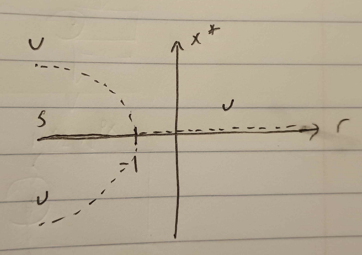
\includegraphics[width=0.5\textwidth]{p1ee.png}
        \end{center}
        \end{itemize}
        \newpage
    \item[(f)] \[\dot{x} = rx + \frac{x^3}{1+x^2}\]
    \paragraph{Solution}\mbox{} 
    \begin{itemize}
        \item Find fixed points:
        \[\dot{x} = f(x)\quad \implies f(x^*) = 0\]
        \[x^*\left(r + \frac{{x^*}^2}{1+{x^*}^2}\right) = 0\]
        \[x^*=0,\quad x^* = \pm \sqrt{\frac{-r}{1+r}}\]
        For the nonzero fixed points to be real, we need $-r/(1+r) \geq 0 \implies -1<r<0$.
        \item Vary parameter $r$ and find bifurcation points:
        \begin{itemize}
            \item $r<-1$: One fixed point at $x^*=0$  
            \item $-1<r<0$: Three fixed points at $x^*=0,\quad x^* = \pm \sqrt{\frac{-r}{1+r}}$
            \item $r=0$: One fixed point at $x^*=0$ 
            \item $r>0$: One fixed point at $x^*=0$ 
        \end{itemize}
        \item Find stability of fixed points:
        \[f'(x) = r + \frac{3x^2(1+x^2)-x^3(2x)}{(1+x^2)^2} = r+\frac{x^2(3+x^2)}{(1+x^2)^2}\]
        \[f'(0) = r\]
        \[f'\left(\pm \sqrt{\frac{-r}{1+r}}\right) = -2r(1+r)\]
            \begin{itemize}
            \item $r<-1$: One fixed point at $x^*=0$  
            \item $-1<r<0$: Three fixed points at $x^*=0,\quad x^* = \pm \sqrt{\frac{-r}{1+r}}$
            \item $r=0$: One fixed point at $x^*=0$ 
            \item $r>0$: One fixed point at $x^*=0$ 
        \end{itemize}
        \newpage
        \item Bifurcation diagram:
        \begin{center}
            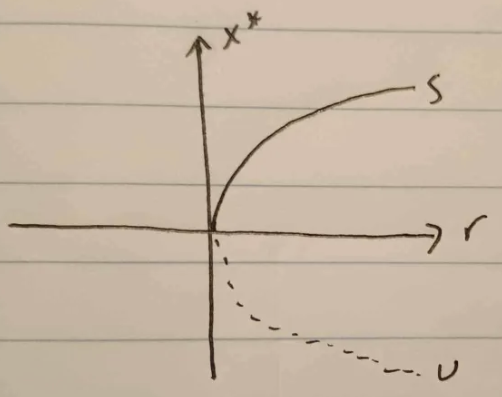
\includegraphics[width=0.5\textwidth]{p1a.png}
        \end{center}
        \item Normal form: 
    \end{itemize}
\end{enumerate}

\subsection*{Problem 2}
\textit{(Problem 3.4.14 in Strogatz)}\\
\textbf{Subcritical Pitchfork.} Consider the system $\dot{x} = rx + x^3 - x^5$, which exhibits a subcritical pitchfork bifurcation (hint: you may want to read about subcritical pitchforks in the book; we did not say much about these in class).
\begin{enumerate}
    \item[(a)] Find algebraic expressions for all the fixed points as $r$ varies.
    \paragraph{Solution}\mbox{} % Write solution here.

    \item[(b)] Sketch the vector fields as $r$ varies. Be sure to indicate all the fixed points and their stability.
    \paragraph{Solution}\mbox{} % Write solution here.

    \item[(c)] Calculate $r_s$, the parameter value at which the nonzero fixed points are born in a saddle-node bifurcation.
    \paragraph{Solution}\mbox{} % Write solution here.
\end{enumerate}

\subsection*{Problem 3}
What can be said about the stability of a fixed point when the derivative at that fixed point is exactly zero? In other words, what is the stability of $x^*$ when
\[f'(x^*) = \frac{df}{dx}(x^*) = 0\,?\]

\paragraph{Solution}
% Write solution here.

\subsection*{Problem 4}
Show that the first-order system
\[\dot{x} = x(1-x^2) - a(1-e^{-bx})\]
undergoes a transcritical bifurcation at $x=0$ when the parameters $a,b$ satisfy a certain equation, to be determined. (This equation defines a bifurcation curve in the $(a,b)$ parameter space.) Then find an approximate formula for the fixed point that bifurcates from $x=0$, assuming that the parameters are close to the bifurcation curve.

\paragraph{Solution}
% Write solution here.

\end{document}
